\documentclass{article}
\usepackage{siunitx}
\usepackage{mathtools}
\usepackage{enumerate}
\usepackage{graphicx}
\usepackage{amssymb}
\sisetup{load-configurations = abbreviations}

\usepackage{fullpage}

\begin{document}

\begin{center}
\textsc{\Large ECE 454 Assignment 2}\\[0.5cm]
\textsc{Amir Benham 20393292, Andrew Svoboda 20369388}\\[0.5cm]
\end{center}

\begin{enumerate}

	\item As we can see in the Figure \ref{fig:q1} we have a network with 5 peers and we want to go from node 0 to node 7.
		
\begin{figure}[ht!]
\centering
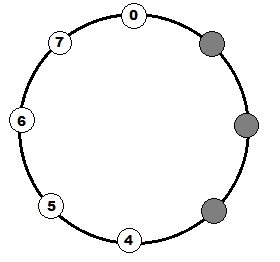
\includegraphics[width=70mm]{q1.png}
\caption{Chord DHT m=3}
\label{fig:q1}
\end{figure}
	
	In this network the finger table of node 0 would look like: \(FT[0]=4, FT[1]=4, FT[2]=0\) which means our next hop would be to node 4. This means that we would have the following situation.
\[
\begin{split}
p & =0, q=4, k=7 \\
q-p&=0 \; and\;  k-p=3 \\
q-p & \ge \frac{k-d}{2} \\
0 & \ge \frac{3}{2} \\
\end{split}
\]
Therefore the equality does not hold.

\item
 \begin{enumerate}
	\item In Figures \ref{fig:dht-2} and \ref{fig:dht-3} below we can see that exactly half of the nodes need to be updated in a worst case scenario. The scenario occurs when the graph is logically separated so that all the nodes exist on one side of the graph. Each node's last finger table pointer all points to the same node in the Chord graph, and so when another node is inserted directly adjacent all other nodes must update their finger tables. Thus the number of nodes that need to update their finger tables is as follows:
\[
\frac{2^m} {2}
\]
\[
=2^{m-1}
\]

	\item Only the predecessor to the item that is being inserted needs to be updated, not including the joining node. For a total of 1 node.
\end{enumerate}

\item The worst case scenario for Chord DHT is when the node that is being looked up is the successor of the nodding doing the look up. In that situation regardless of what m is or regardless of the orientation of the nodes the number of hops will be linear relative to m. 

\item For this solution we need to introduce a few new functions. First we will introduce a function, \( itob()\), that converts an integer to its binary representation. We will need the reverse of that function \(btoi()\). We will also need a function, \(concat()\), that will combine two binary values ie. \(Concat(100,010)\) should result in 100010.  We will also need the reverse of the concat function, we will call it \(split()\) which takes one binary value and splits it down the middle and returns the two tokens ie. \([b1,b2]=split(someBinaryString)\), where \( b1\) and \(b2\) are the most significant and least significant bits respectively.

\[
\begin{split}
(i,j) & \rightarrow n \\
n & = \text{btoi}(\text{concat}(\text{itob}(i),\text{itob}(j)) \\
n & \rightarrow(i,j) \\
[b1,b2] & = \text{split}(n) \\
i & = \text{btoi}(b1) \\
j & = \text{btoi}(b2) \\
\end{split}
\]
	
\item
There are two possible ways that a route can be created between Q and P either Q chooses P or P chooses Q. The total number of routes are \( \binom{n-1}{c-1}\)

\[
\therefore P = \frac{2}{\binom{n-1}{c-1}}
\]

\item Using the bully election system the worst case scenario would be if the node with the lowest id sends out an election message to \(n-1\) nodes and gets \(n-1\) OK messages back. Then the node with the second lowest node sends out \(n-2\) messages out and gets \(n-2\) messages back and so on. When the last node sends out the election message and gets no OK message back, it will send out a coordinator message out to let everyone know that it is the new super node .The end result would be \(2*(n-1)+2(n-2)+2(n-3)... 2*1= n*n-1 = O(n^2)) \).

The worst case scenario for Ring election would be if every node started an election at the same time. So that is \(n\) messages that get passed around \(n-1\) times and each message grows to a size of \(n\). After that goes around they will all send out the coordinator message with a list of every living process in it. So that is \(n\) messages of size \(n\) being sent out. In the end we get a total of  \(n*(n-1)*n+n*n-1*n =O(n^3)\)


\item One way to get rid of duplicate messages as soon as possible would be to add a time stamp to the election message. After a node sees the message they will keep track of it and if another message gets past to them that has a new a time stamp the node will not forward it. The node will reset the time stamp after it receives the response from the initiator. If we do not want to modify the election message by adding a time stamp to it the same concept can be applied by counting how large the list in the message is but this method does not work as well.


\begin{figure}[ht!]
\centering
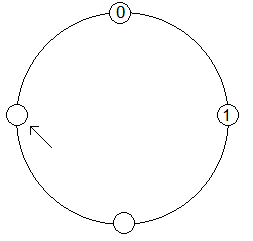
\includegraphics[width=70mm]{q2a_m2.png}
\caption{Chord DHT m=2}
\label{fig:dht-2}
\end{figure}


\begin{figure}[ht!]
\centering
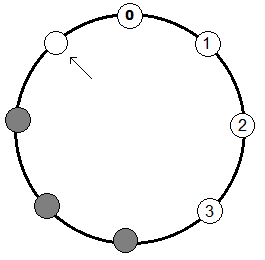
\includegraphics[width=70mm]{q2a_m3.png}
\caption{Chord DHT m=2}
\label{fig:dht-3}
\end{figure}

\end{enumerate}

\end{document}
